
\documentclass[11pt,a4paper]{article} %% 1.Ebene = chapter, headings

\usepackage[utf8]{inputenc} 
\usepackage[T1]{fontenc} 
\usepackage{lmodern}
\usepackage{tcolorbox}

\usepackage[german]{babel}


\setlength{\parindent}{0pt}
\setlength{\parskip}{1ex plus 0.5ex minus 0.5ex}

\usepackage{amsmath} 


\usepackage{graphicx} 

\usepackage[section]{placeins}
\usepackage{booktabs}


\usepackage{hyperref}
\hypersetup{
	colorlinks,
	citecolor=red,
	filecolor=black,
	linkcolor=black,
	urlcolor=black}
\graphicspath{}

\begin{document}



{
	\centering 
	\large 
	Physiklabor für Anfänger*innen \\
	Ferienpraktikum im Sommersemester 2018 \\[4mm]
	\textbf{\LARGE 
		Versuch 17: Physikalisches Pendel, Trägheitsmomente und Steinerscher Satz
	} \\[3mm]
	(durchgeführt am 17.09.2018 bei Adrian) \\
	Ye Joon Kim, Marouan Zouari\\
	\today \\[10mm]
}
\tableofcontents
\newpage
\section{Einleitung}
Mit dem Trägheitsmoment eines Physikalischen Pendels kann man seine Periode vorhersagen. Dafür wird es benötigt, die Bewegungsgleichung des Pendels aufzustellen. 
\\\
Die Definition des Drehmoments ist:
\begin{equation}
\vec{M} = \vec{F}\times \vec{r}
\end{equation}
Wobei $\vec{F}$ die Kraft und $\vec{r}$ der Ortsvektor. Das Drehmoment lässt sich auch schreiben als:
\begin{equation}
\vec{M} = I \cdot \ddot{\varphi}
\end{equation}
Wobei $I$ das Trägheitsmoment und $\varphi$ die Drehwinkel. 

Die auf dem Stab wirkende Kraft $F_G$ (Die zur Stab  senkrechte Komponente) ist:
\begin{equation}
\vec{F_{G\perp}} = m\vec{g}\sin(\varphi)
\end{equation}
Der Betrag der auf dem Stab wirkenden Trägheitsmoment ist deshalb:
\begin{equation}
M = xmg\sin(\varphi)
\end{equation}
Wobei $x$ der Abstand von dem Aufhängepunkt zum Schwerpunkt ist. Gleichung (2) und (4) können gleichgesetzt werden, um
$$ I \cdot \ddot{\varphi} = xmg\sin(\varphi)$$ 
zu liefern. 

Für kleine Winkel ist $\sin(\varphi) \approx \varphi$, und nach Umformen der Gleichung bekommt man:
$$ \ddot{\varphi} - \frac{xmg}{I} \varphi = 0$$
, was eine Differentialgleichung eines harmonischen Oszillator mit $\omega^2 = \frac{xmg}{I}$ darstellt. 

Der Frequenz eines Drehpendel wird ähnlich berechnet. Mit $M = -D\varphi$ und $M = I\ddot{\varphi}$ gilt:
$$-D\varphi = I\ddot{\varphi}$$
,was wieder eine Differenzialgleichung eines harmonischen Oszillators darstellt, mit 
\begin{equation}
\omega = \sqrt{\frac{D}{I}}
\end{equation}



Zur Bestimmung des Trägheitsmoments eines Körpers wird die folgende Formel benutzt:
\begin{equation}
I = \int r_\perp^2 dm
\end{equation}

Für den ersten Versuchsteil ist es notwendig das Trägheitsmoment eines Zylinderförmigen Stabes zu bestimmen. Zur Erleichterung der Rechnung wird das Integral in Zylinderkoordinaten durchgeführt. Mit $dm = \rho dV$ ist das Integral:
$$I = \rho \int_{0}^{2\pi} \int_{-L}^{0} \int_{0}^{r} \sin^2(\phi)r^3 + z^2r dr dz d\phi$$ 
,was 
\begin{equation}
I_\textrm{Pendel} = \frac{1}{4}Mr^2 +\frac{1}{3}ML^2
\end{equation}
ergibt. Wobei $r$ der Radius und $L$ die Länge des Stabes sind. 

In dem zweiten Teil muss das Trägheitsmoment der Kreisscheibe bestimmt werden. Das Rechnen mit der Formel (6) ist einfach, da die Scheibe Zylinderförmig ist. Das Trägheitsmoment ist deshalb:
$$ I_\textrm{Scheibe} = \rho \int_{0}^{2\pi} \int_{-L}^{0} \int_{0}^{r} r dr dz d\phi $$
\begin{equation}
= \frac{1}{2}mr^2
\end{equation}
Wobei $r$ der Radius der Scheibe ist. 
\section{Ziel des Versuchs}
In dem ersten Versuchsteil wird die Schwingungsdauer eines physikalischen Pendels gemessen und mit dem theoretischen Wert verglichen. 
\\\
In dem zweiten Versuchsteil wird die Zusammenhang von dem Abstand zwischen die Kreisscheibe und den Zentrum des Drehpendels mit der Schwingungsdauer untersucht. 

\section{Versuchsdurchf"uhrung und Aufbau}
(Siehe Abbildung auf Seite 5.)

 

\begin{figure}[h]
	\centering
	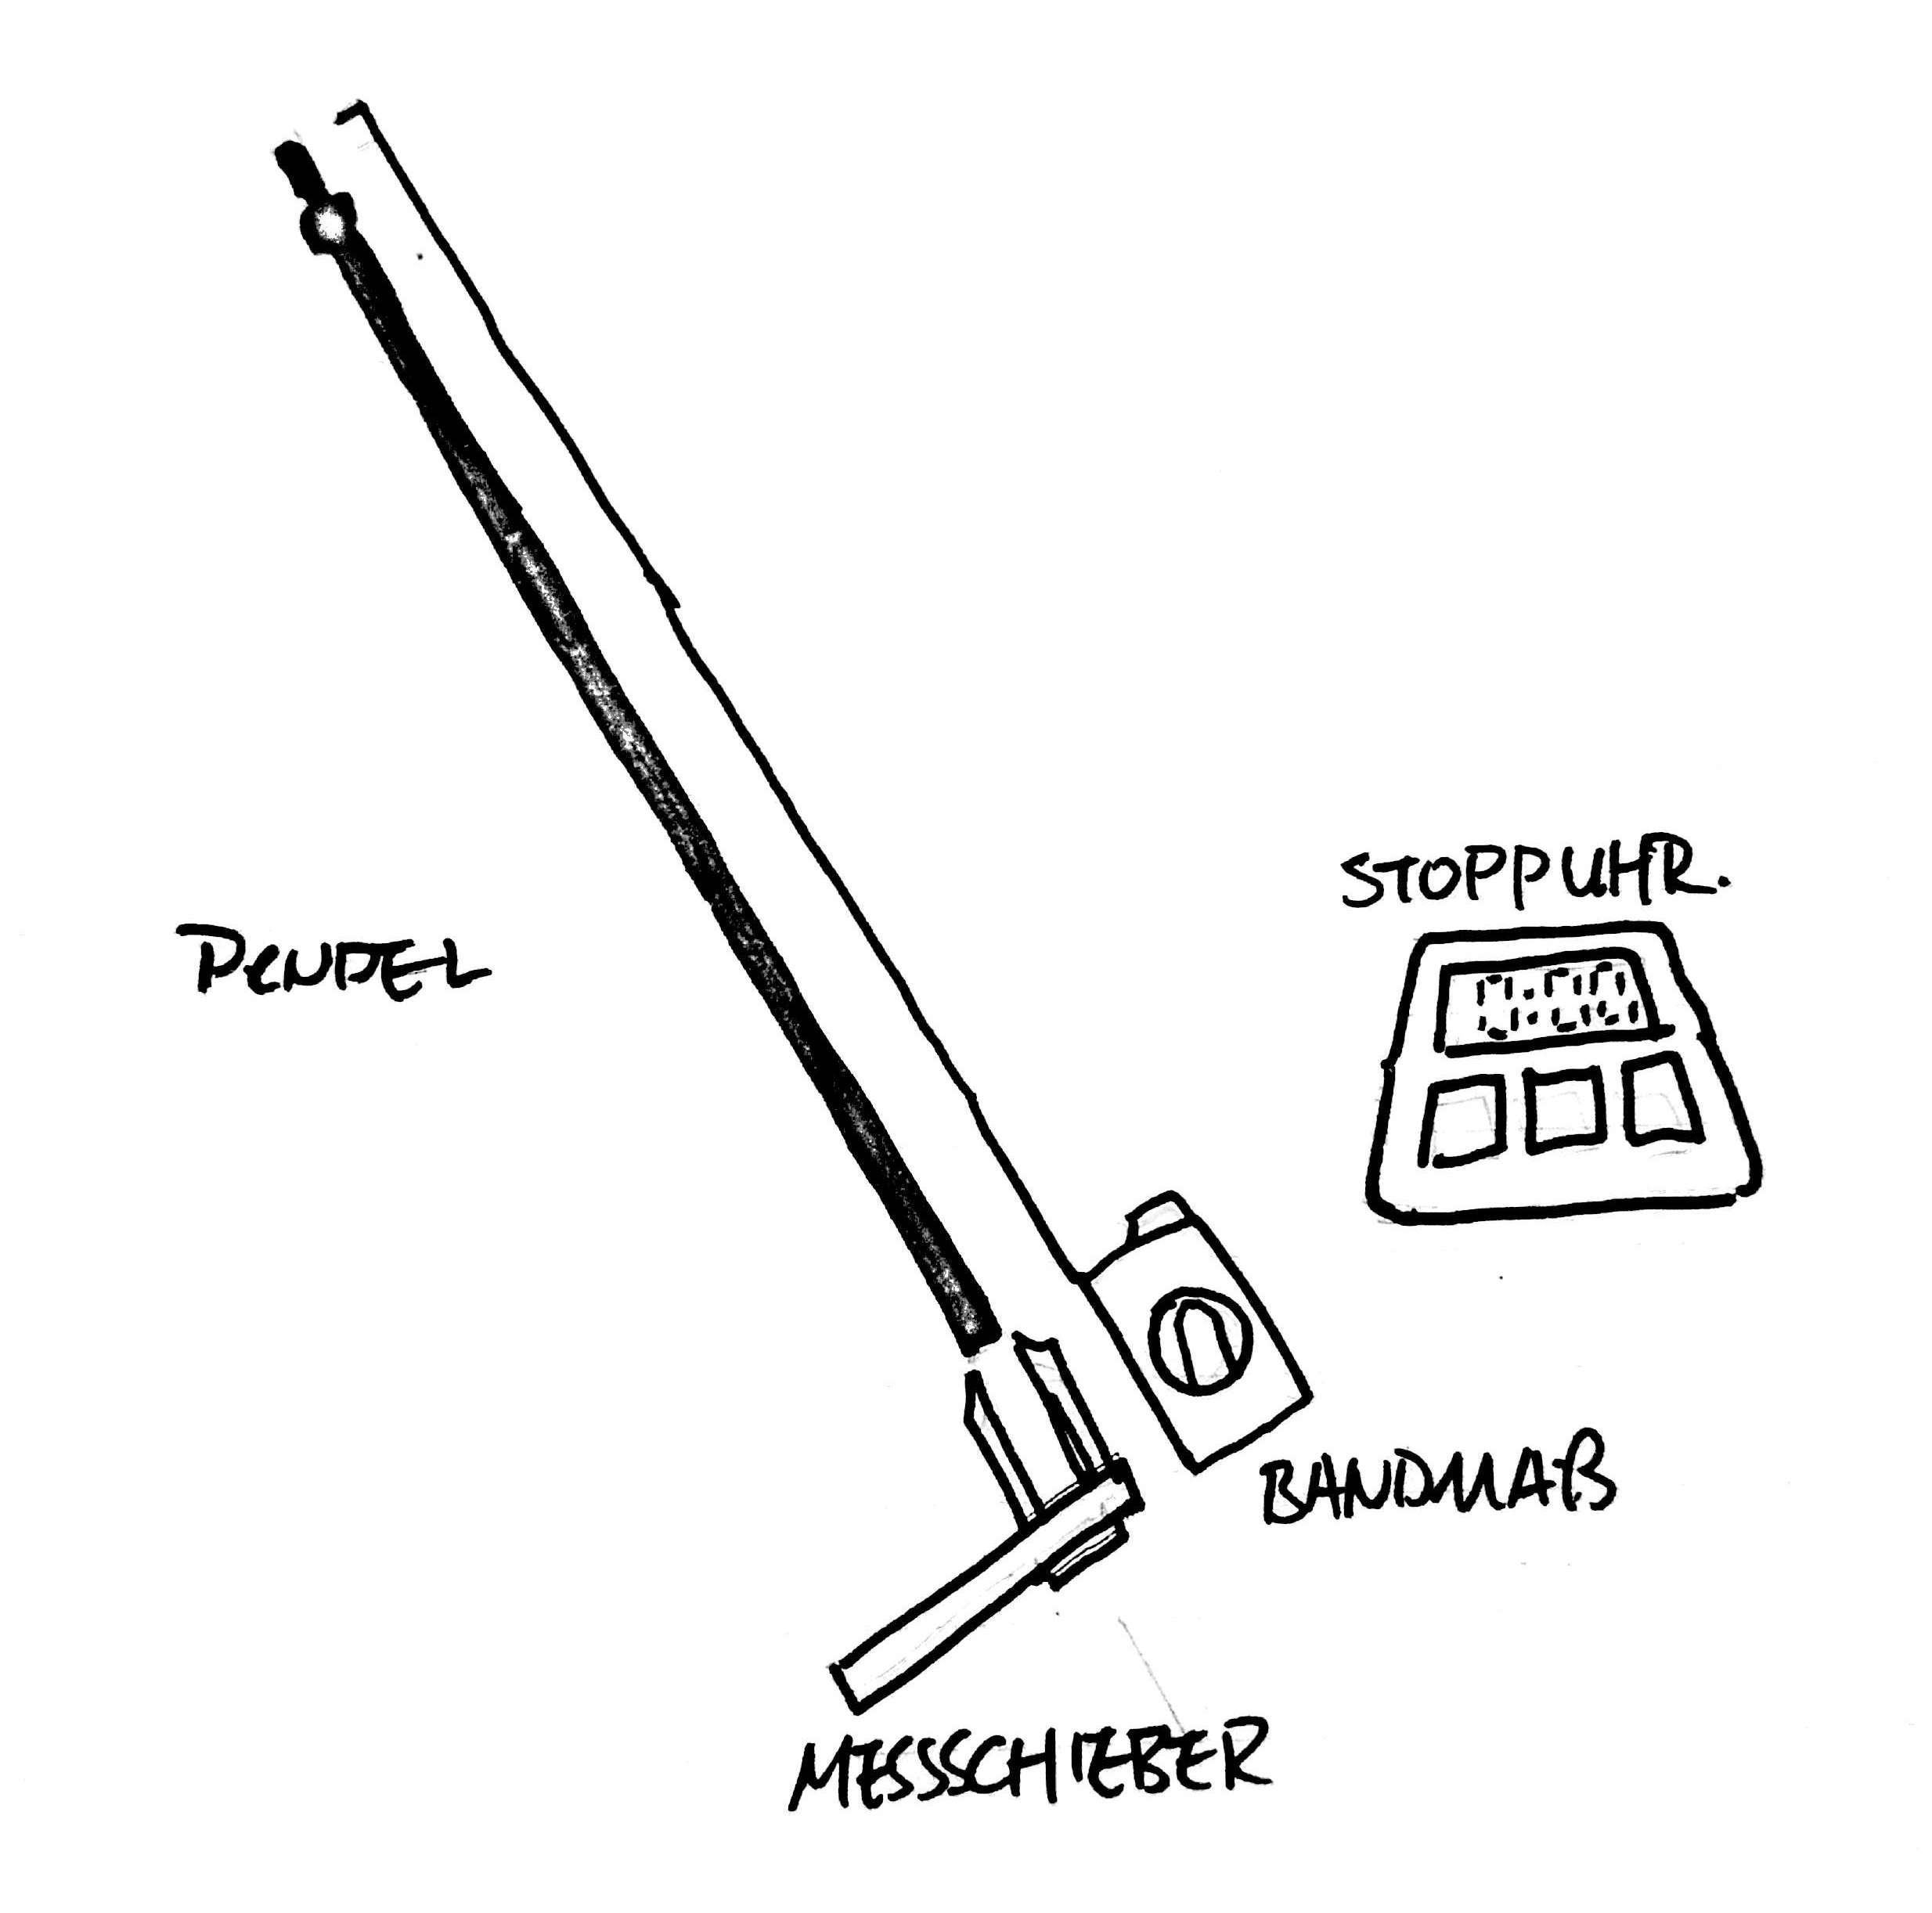
\includegraphics[scale=0.1]{Abb1}
	\caption{Aufbau zur Messung der Schwingungsdauer eines physikalischen Pendels}
	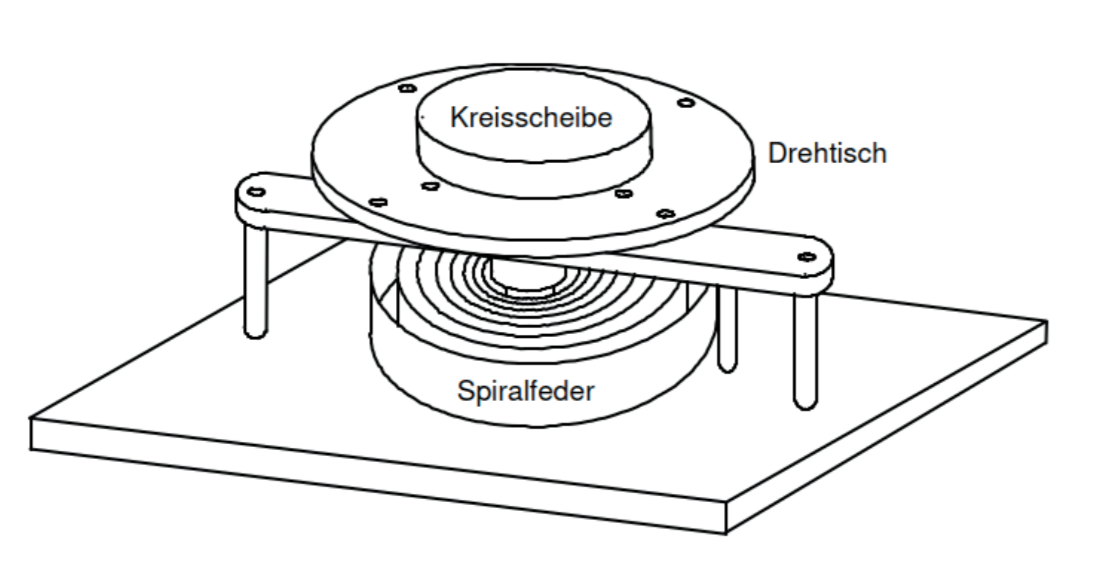
\includegraphics[scale=0.5]{Abb2}
	\caption{Aufbau zur Messung der Schwingungsdauer eines Drehpendels (Quelle
		:Versuchsanleitungen AP-1)}
	
	
	
\end{figure}

\subsubsection{Physikalisches Pendel}
Zur Messung der Periode eines Physikalisches Pendel wurde einen Zeitmesser benutzt. Mit einem Bandmaß wurde die Länge des Stabes und mit einem Messschieber wurde den Durchmesser des Stabes gemessen. 

Der Stab wurde dann leicht aufgehoben und losgelassen. Die Zeitmessung wurde angefangen, als der Stab an dem roten senkrechten Stab im Mitte vorbeiging, und geendet, am dritten Mal, dass der Stab an dem roten Stab vorbeiging (Da das zweite Mal entspricht eine halbe Periode). Die einzelne Zeitdauer wurden aufgenommen. Der Prozesse wurde dreißig mal wiederholt. 

Für die alternative Methode wurde der Stab aufgehoben und losgelassen, und die Zeitmessung wurde wie vorher angefangen. Es wurde dreißig Schwingungen gewartet, bis die Uhr gestoppt wurde. Die gesamte Zeitdauer wurde dann aufgenommen. 


\subsubsection{Das Drehpendel}
Der Durchmesser der Kreisscheibe wurde mit einem Messschieber gemessen. Der Drehtisch wurde dann ohne die Kreisscheibe gedreht und losgelassen. Ähnlich wie in dem ersten Teil wurde die Zeitmessung gestartet, als die Kennzeichnung auf dem Drehtisch an der ursprünglichen Position vorbeigegangen war. Die Uhr wurde gestoppt als die Kennzeichnung dreimal an der ursprünglichen Position vorbeigegangen war. Der Prozesse zehn mal wiederholt. Dann wurde die Schwingungsdauer mit der Kreisscheibe auf dem Drehtisch gemessen. 

Danach wurde die Kreisscheibe von dem Zentrum des Drehtisches versetzt, und die Schwingungsdauer des Drehpendels gemessen. Der Abstand zwischen das Zentrum des Drehtisches und der Kreisscheibe wurde dadurch gemessen, indem man mit einem Messschieber die Abstände zwischen die Löcher auf dem Drehtisch misst.


\FloatBarrier
\section{Auswertung und Fehleranalyse}




\subsection{Bestimmung der theoretischen Schwingungsdauer}
Wie in der Einleitung erwähnt, ist der Kreisfrequenz eines physikalischen Pendels $\omega = \sqrt{\frac{xmg}{I}}$. Das Einsetzten von Gleichung (6) in diesem Ausdruck liefert:
$$\omega = \sqrt{\frac{xg}{\frac{1}{4}r^2+\frac{1}{3}L^2}}$$
Und da $\omega = \frac{2\pi}{T}$ ist die theoretische Schwingungsdauer:
$$T = 2\pi \sqrt{\frac{\frac{1}{4}r^2+\frac{1}{3}L^2}{xg}}$$
Die Theoretische Schwingungsdauer von der Pendel ist deshalb:
$$(1,15\pm 0,03) \textrm{ s}$$
\begin{tcolorbox}[colback=white]
	\subsubsection{Beispielrechnungen}
	Zur Berechnung der Unsicherheit von der theoretischen Schwingungsdauer wurde die Gauß'sche Fehlerfortpflanzung benutzt. Mit
	$$f(x,r,L) = 2\pi \sqrt{\frac{\frac{1}{4}r^2+\frac{1}{3}L^2}{xg}}$$
	sind:
	$$\frac{\partial f}{\partial x} = -\frac{\frac{1}{4}r^2+\frac{1}{3}L^2}{2g\sqrt{\frac{\frac{1}{4}r^2+\frac{1}{3}L^2}{gx}}x^2} $$
	$$\frac{\partial f}{\partial r} = \frac{\frac{1}{4xg}r}{\sqrt{\frac{\frac{1}{4}r^2+\frac{1}{3}L^2}{xg}}}$$
	$$\frac{\partial f}{\partial L} = \frac{\frac{1}{3xg}L}{\sqrt{\frac{\frac{1}{4}r^2+\frac{1}{3}L^2}{xg}}}$$
	Aber da die Beträge von $\frac{ \partial f}{\partial x} \Delta x$ und $\frac{\partial L}{\partial L} \Delta L$ mehr als 100-Mal größer sind als der andere Betrag, wurde der $\frac{ \partial f}{\partial r} \Delta r$ vernachlässigt. Deshalb ist die Unsicherheit der Schwingungsdauer:
	$$\Delta T = \sqrt{ 
		(\frac{ \partial f}{\partial x} \Delta x)^2
		+(\frac{\partial L}{\partial L} \Delta L)^2
	}
	$$
	
\end{tcolorbox}

Das Einsetzen der Abmessungen in die Formel (8) liefert das Trägheitsmoment der Kreisscheibe. 
$$ I = 0,00202 \pm 0,00001$$
Seine Unsicherheit wurde mit der vereinfachten Formel für Produkte und Quotienten berechnet, nämlich:
$$\vert\frac{\Delta I}{I}\vert = \frac{1}{2}\sqrt{(\frac{\Delta m}{m})^2+(2\frac{\Delta r}{r})^2}$$


\subsection{Bestimmung der Schwingungsdauer eines Physikalischen Pendels}
In dem ersten Teil wurden 30 Einzelmessungen durchgeführt. Der Mittelwert und seine Standardunsicherheit lauten:
$$ (1,553 \pm 0,002) \textrm{ s}$$
Danach wurde die Zeitdauer für 30 Schwingungsdurchgänge gemessen. Die mittlere Dauer einer einzelnen Schwingung und ihre Unsicherheit sind:
$$ (1,60 \pm 0,05) \textrm{ s}$$
\begin{tcolorbox}[colback=white]
\subsubsection{Beispielrechnungen}
Die Mittelwerte lassen sich mit der folgenden Formel berechnen:
$$\bar{x} = \frac{1}{n} \sum_{i=1}^{n} x_i$$

und die Standardunsicherheit:

$$s_x = \sqrt{\frac{\sum_{i=1}^{n}(x_i-\bar{x})^2}{n-1}} $$

Bei der zweiten Messung gab es keine Standardunsicherheit, deswegen wurde der Messfehler durch einen Faktor $\sqrt{n}$ geteilt, wobei $n$ die Anzahl Schwingungen ist. 


\end{tcolorbox}

\subsection{Bestimmung der Schwingungsdauer eines Drehpendels}
Die Durchschnittliche Schwingungsdauer des Drehpendels ohne die Kreisscheibe ist:
$$ T = (2,163 \pm 0,02) \textrm{s} $$

Mit demselben Prozesse lassen sich die Schwingungsdauer des Drehpendels mit verschiedenen Abstände von der Kreisscheibe bestimmen. 


\begin{table}[h]
	\centering
	\begin{tabular*}{0.99\textwidth}{@{\extracolsep{\fill}}c|ccc}
		\toprule
		Abstand ($d$) & $\bar{T}$ & $u_{\bar{T}}$  \\
		m & s & s   \\
		\bottomrule
		0,0000 & 2,39 & 0,01 \\
		0,0150 & 2,42 & 0,01 \\
		0,0300 & 2,57 & 0,02 \\
		0,0600 & 2,98 & 0,01 \\
		0,0900 & 3,56 & 0,01 \\
		\bottomrule
	\end{tabular*}
	\caption{Die Werte für die durchschnittlichen Schwingungsdauer für verschiedene Abstände und deren  Unsicherheiten}
	\label{tabelle}
\end{table}
\FloatBarrier
Die Unsicherheiten der Abstände sind $1 \cdot 10^{-4}$ m. 

Das Rechnungsverfahren ist genau wie im ersten Teil erläutert. 

Die Werte für $d^2$ und $\bar{T}^2$ wurden in einer Graph eingetragen. Die Berechnung der linearen Regression wurde mit einem Excel-Dokument und die Graph mit dem Programm Logger-Pro gemacht. 
\begin{figure}[h]
	\centering
	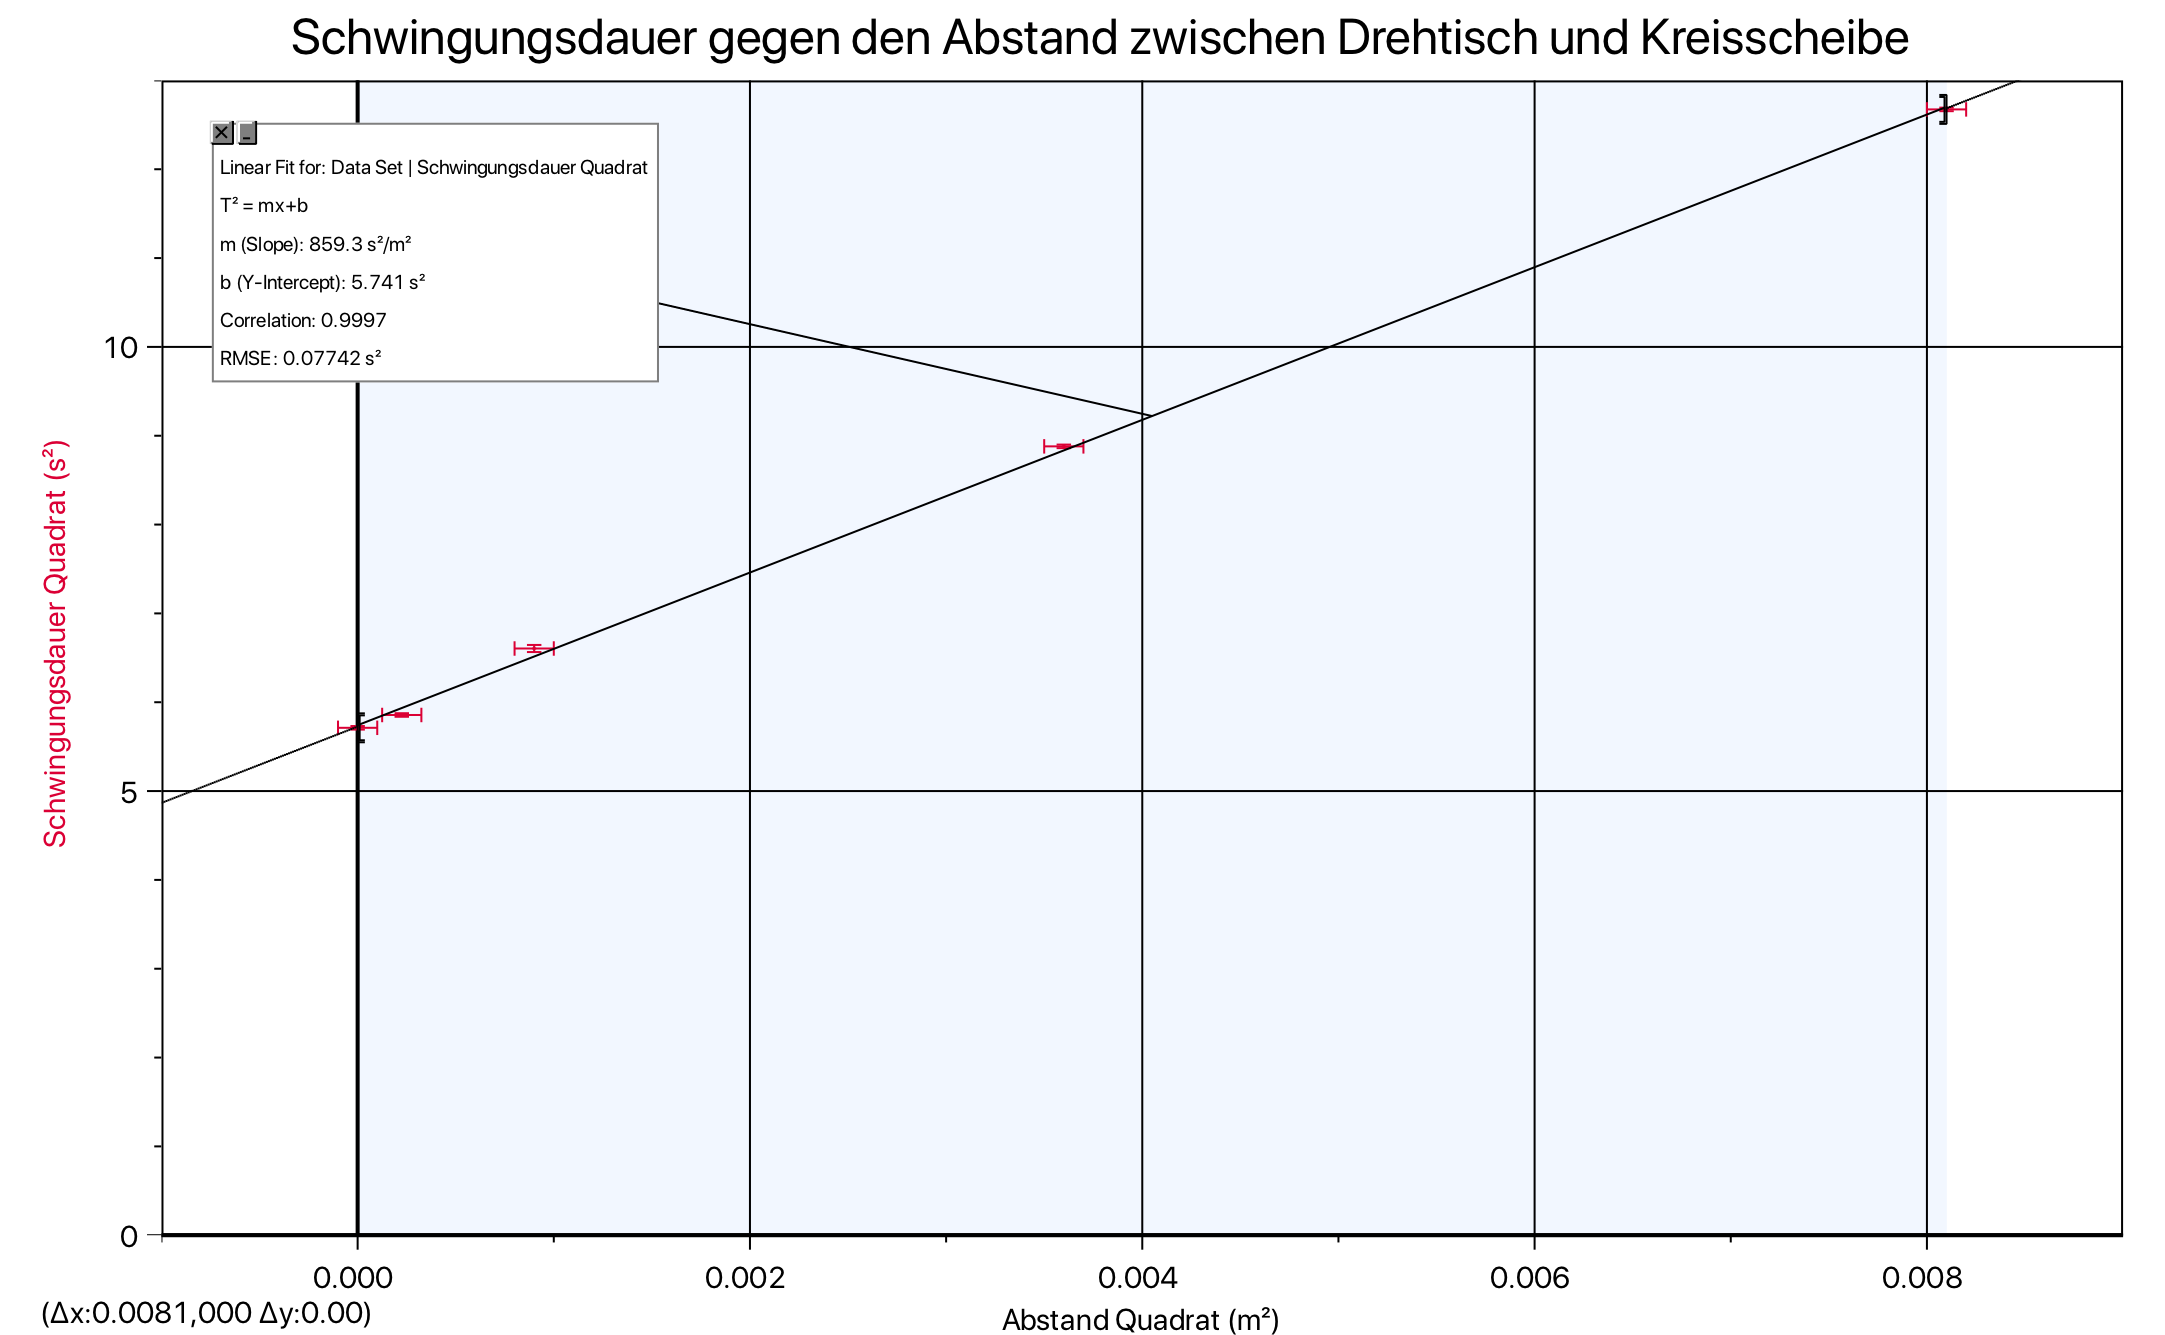
\includegraphics[width=\linewidth]{Graph1}
	\caption{Graph von $T^2$ als Funktion von $d^2$}
\end{figure}
Die berechnete lineare Regression ist:
$$a+bx = 5,71 + 859x$$
mit den Unsicherheiten $u_a = 0,05 \textrm{s}^2$ und $u_b = 11 \textrm{s}^2 \textrm{m}^{-2}$

Aus der Steigung und dem Steiner'schen Satz kann das Gesamt-Trägheitsmoment bestimmt werden. Der Steiner'sche Satz lautet:
$$ I = I_\textrm{cm} + md^2 $$
Mit dem Umformen der Gleichung (5) und das Einsetzen in der obigen Formel liefert:
$$T^2 = \frac{I_0}{D} + \frac{m}{D}d^2$$
Die Steigung ist deshalb $\frac{m}{D}$, und dadurch lässt sich der Wert von $D$ berechnen. 
$$D = (0,00135 \pm 0,00002) \textrm{  Nm}^{-1}\textrm{rad}^{-1}$$

Und mit dem Achsenabschnitt $\frac{I_\textrm{cm}}{D}$ das Trägheitsmoment der gesamten Anordnung. 
$$ I_\textrm{cm} = (0,0077 \pm 0,0001) \textrm{ kgm}^2 $$

Für beide Unsicherheiten wurde die vereinfachte Formel für Produkte und Quotienten angewendet.

Jetzt kann das Drehmoment des Drehtisches bestimmt werden, indem man das Trägheitsmoment der Kreisscheibe von dem Gesamt-Trägheitsmoment subtrahiert. 

$$I_\textrm{Tisch} = (0,0057 \pm 0,001) \textrm{ kgm}^2 $$

Die Unsicherheit des Trägheitsmoments der Kreisscheibe wurde vernachlässigt, da es ein Zehntel von der von dem Drehtisches war. 




\section{Diskussion der Ergebnisse}
\subsection{Diskussion der Werte}
Die Schwingungsdauer des physikalischen Pendels für beide Messmethoden waren:
$$(1,553 \pm 0,002) \textrm{s}$$
$$(1,60 \pm 0,05) \textrm{s}$$
Deren Differenz, 0,047 s, ist mehr als 20-mal der Standardunsicherheit des ersten Ergebnisses, deshalb stimmen beide Werte nicht überein und sind nicht verträglich. 
\\\
Das erste Ergebnis liegt innerhalb des Fehlers von dem zweiten Wert, aber das ist von keiner großen Bedeutung, da die relative Unsicherheit von dem zweiten Messwert ungefähr 20-mal größer ist als die des ersten Werts. Ein möglicher Grund dafür ist die gegebene systematische und statistische Fehler. 

Im Vergleich mit dem theoretischen Wert, $1,63 \pm 0,03$ s, sind beide Werte niedrig. Nur der zweite Messwert stimmt mit dem theoretischen Wert überein, da beide Werte innerhalb eine Standardunsicherheit voneinander liegen, und die relative Unsicherheit beträgt 0,03, deshalb ist dieses Ergebnis auch Bedeutungsvoll. 
\\\
Auf der anderen Seite, liegt die theoretische Wert außerhalb mehr als 30 Standardabweichungen von dem ersten Wert, aber das impliziert nicht, dass der Bedeutungslos ist oder dass der Wert nicht zu vertrauen ist. Obwohl die theoretische und gemessene Werte weit auseinander liegen, ist die Streuung des gemessenen Wert sehr klein. 
\\\
Die relative Unsicherheit des ersten Werts ist 0,0012, und das impliziert, dass es einen systematischen Fehler gab, der alle Messwerte nach unten verschoben hatten. 

\subsection{Systematische und statistische Fehler}
\textbf{Bei dem physikalischen Pendel} war der Punkt, worauf das Pendel gehängt wurde, nicht ganz fest. Das f"uhrt zu seitigen Schwingungen, die  statistische Fehler bei der Schwingungsdauermessungen bringen könnten. 
\\\
Außerdem rundet die Stoppuhr die angezeigten Zeiten auf unbekannte weise, möglicherweise in Abstände von 0,03 Sekunde. Deswegen kann die Stoppuhr nur bestimmte Werte anzeigen, aber das war Vernachlässigt, da die Unsicherheit, die von der Reaktionszeit resultiert, viel größer war. 
Ein systematischer Fehler entsteht aus der Verwendung der Kleinwinkelapproximation, da wenn die Winkel außerhalb des Intervalls der Approximation liegen, wird der gesamte berechnete Wert größer als der wirkliche Wert sein.

\textbf{Bei dem Drehpendel} hängt die Abschätzung der Anzahl Schwingungen und deren Dauer von der Reaktionszeit und der Position des Beobachters ab. entsteht davon statistische Fehler.
\\\
Wie beim 1. Teil, formt die Kleinwinkelapproximation einen systematischen Fehler.
\subsection{ M"ogliche Verbesserungen}
Das Pendel sollte so befestigt werden, dass es nur einen Freiheitsgrad hat, der in der Richtung der Schwingungen liegt. Auch sollten die Befestigungspunkte geschmiert werden, um die Auswirkungen der Reibungen zu minimieren.
\\\
Die Schmierung ist auch eine mögliche Verbesserung f"ur den Versuch mit dem Drehpendel.
\\\
Es wäre auch besser, ein automatisches System zu benutzen, das die Anzahl und die Dauer der Schwingungen automatisch bestimmt.
\section{Literatur und Bildquellen}
,,Versuchsanleitung zum Physiklabor für Anfänger*innen.'' Albert-Ludwigs-Universität Freiburg. 








\end{document}


